\section{Introduction}

In-situ processing is a solution to solve the gap between the computation and communication performance of HPC infrastructure for several decades\cite{childs2012situ}. Several works are focusing on the in-situ solution and how to make it leverage the scientific application\cite{bauer2016situ,oldfield2014evaluation}. Typical subtypes for simulation-analyzing-visualization application\cite{childs2012situ}: post-processing , co-processing, concurrent processing, Hybrid. There are other dimension to divide the application such as if they are running within same program \cite{dreher2017decaf}. Based on those definitions of the concept of in-situ, in-transit, hybrid scientific application, we clarify properties of every solution by several  essential underlying perspective which are shown in Figure 1, to be more specific:

\begin{figure} 
\centering
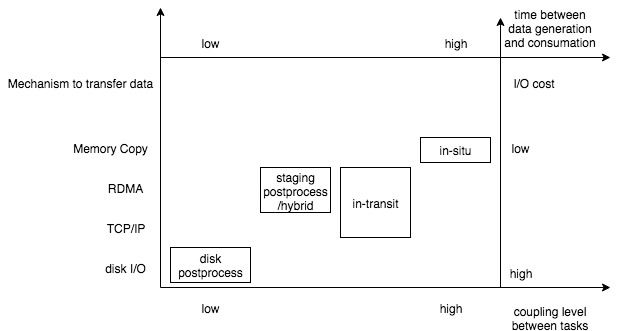
\includegraphics[width=.95\linewidth]{./figure/application_classification.jpg}
\caption{classification for scientific application running pattern}
 \label{fg:state}
\end{figure} 

The post-processing analysis with disk using is the naive and traditional way to compose a scientific workflow. The visualization/simulation will load the disk data outputted by previous dependent tasks. There is a minimum degree of coupling (largest independency) between two tasks in this context because the task of data produces don't need any information about the task which consuming data. 

The post-processing analysis with staging server works by constructing pipeline based on data management service. The I/O cost can be decreased by leverage the function of staging service, but it required some modification of simulation in order to using API provided by staging service. Further optimization could be adopted in staging service to decrease I/O cost relatively such as data locality and placement strategies.

If tasks are composed within one program, the data could also be transferred by the network such as using MPI or other dedicated network library (in-transit workflow) this will increase the coupling level and instrument simulation code in much higher level. The data could also be transformed by the specialized adaptor to transform the data structure.

Within one program, the data could also be transferred by much higher level coupling namely run visualization code synchronously after each iteration which increases coupling level and data transfer speed (in same memory space).

There is no absolute preference  solution for any using context and every solution has tradeoff in Figure 1, in situ and in transit analysis does not displace the need for post-post processing pattern even if there is large I/O cost for scientific workflow\cite{bauer2016situ}.  For in-situ  and in-transit application the disadvantage is that the in-situ code will influence the performance of the simulation, not all coupling task is suitable for the in-situ pattern. The Hybrid workflow is more useful in real scientific workflow which is composed of different level of coupling task inorder to leverage the advantage for specific task and minimize their disadvantages. One challenge is how the workflow to support the complex integration of application patterns in Figure 1. Even though there are all kinds of work focusing on the intermediate component such as data staging service or in-situ adaptor to leverage specific scenarios (we will discuss this in Background and related work) there are few works explore how to support hybrid pattern in portable, flexible and scalable way(the aim of the experiments).

Our work provides a method based on event programming to leverage the hybrid scientific pattern including in-situ and in-transit part, we also implement an event driving workflow tool to compose the scientific application and evaluate its effectiveness in Experiment part. We also show the potential to combine this workflow with low-level resource scheduler system to leverage whole running task of the scientific workflow (more detailed after experiments finishing, maybe provide some good practice to implement the hybrid workflow including in-situ in-transit and post-processing)

The rest paper is organized as follows, Section \uppercase\expandafter{\romannumeral2} introduce the background and the related work of event-driven workflow, Section \uppercase\expandafter{\romannumeral3} introduce the design and implementation of workflow framework. Section \uppercase\expandafter{\romannumeral4} presents the experiments to show the performance and effectiveness of the framework. Section \uppercase\expandafter{\romannumeral5} introduce the conclusion and the future work of the work.
